\section{Casos de Uso}
A partir de los requerimientos ya definidos, se desarrolla el diagrama de casos de uso, en el que se representan las interacciones entre actores y las partes más importantes del software a desarrollar. Luego, se realizan las especificaciones de los casos de uso definidos en el diagrama.
\subsection{Diagrama de Casos de Uso}
\begin{figure}[H]
	\centering
	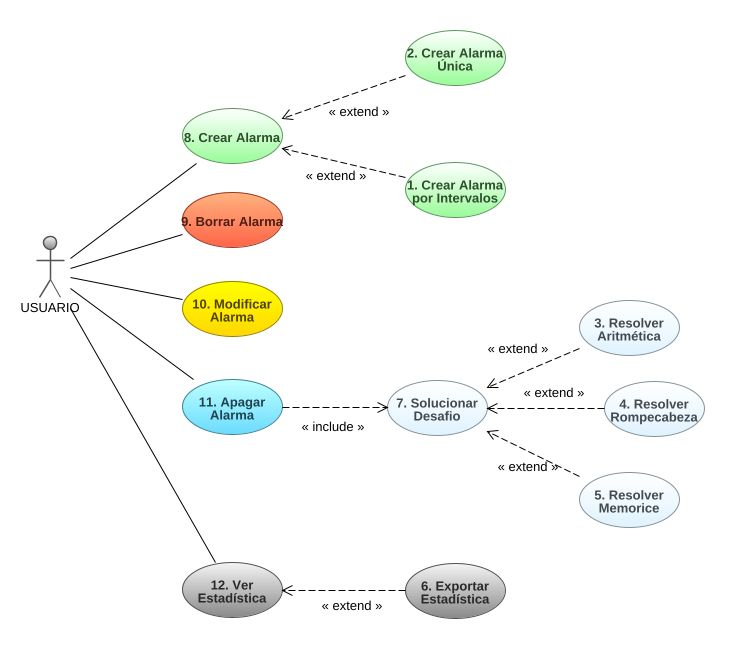
\includegraphics[width=\textwidth]{img/Diagrama Casos de Uso.jpg}
	\caption{Diagrama de Casos de Uso}
	\label{fig:Diagrama de Casos de Uso}
\end{figure}
\newpage

\subsection{Especificación de Casos de Uso}
En esta sección se presenta la especificación de los casos de uso introducidos por el diagrama de casos de uso.


\begin{table}[H]
    \centering
    \caption{Caso de Uso Nº1: Crear Alarma por Intervalos}
    \begin{tabular}{| p{0.4\linewidth} | p{0.4\linewidth} |}
        \hline
        \multicolumn{2}{|l|}{\textbf{Caso de Uso Nº1:}  Crear alarma por intervalos} \\
        \hline
        \multicolumn{2}{|l|}{\textbf{Resumen:}  El usuario crea una alarma dentro de un intervalo de tiempo.} \\
        \hline
        \multicolumn{2}{|l|}{\textbf{Frecuencia:}  Ilimitada} \\
        \hline
        \multicolumn{2}{|l|}{\textbf{Actores:}  Usuario} \\
        \hline
        \multicolumn{2}{|l|}{\textbf{Precondiciones:}} \\
        \hline
        \multicolumn{2}{|l|}{\textbf{Descripción del flujo normal (escenario exitoso)} } \\
        \hline
        \textbf{Responsabilidad del actor} & \textbf{Responsabilidad del sistema}\\
            & 1. Habilitar campo ``Hora inicio".\\
            & 2. Habilitar campo ``Hora término". [exc01]\\
            & 3. Habilitar campo ``número de alarmas". \\
            & 4. Habilitar opción ``Desafío aritmético".\\
            & 5. Habilitar opción ``Desafío rompecabeza".\\
            & 6. Habilitar opción ``Desafío memorice".\\
        7. Ingresar ``Hora inicio". &\\
        8. Ingresar ``Hora término". &\\
        9. Ingresar ``Frecuencia". &\\
        10. Seleccionar una de las opciones (“Desafío aritmético”, “Desafío rompecabeza”, “Desafío memorice”) &\\
            & 11. Habilitar opción ``ingresar alarma''.\\
            & 12. Crear alarma por intervalos.\\
            & 13. Fin del caso de uso. \\
        \hline
        \multicolumn{2}{|p{0.8\linewidth}|}{
            \textbf{Excepción:}
            \begin{itemize}
                \item \textbf{[exc01]:} Intervalo incorrecto. Se muestra un mensaje de advertencia “la hora de término tiene que ser mayor a la de inicio”.
            \end{itemize}}\\  
        \hline
        \multicolumn{2}{|l|}{\textbf{Poscondición:}  Alarma por intervalos creada.} \\
        \hline
    
    \end{tabular}    
    
    \label{table:1}
\end{table}

\begin{table}[H]
    \centering
    \caption{Caso de Uso Nº2: Crear Alarma Única}
    
    \begin{tabular}{| p{0.4\linewidth} | p{0.4\linewidth} |}
        \hline
        \multicolumn{2}{|l|}{\textbf{Caso de Uso Nº2:} Crear alarma única} \\
        \hline
        \multicolumn{2}{|l|}{\textbf{Resumen:} El usuario crea una alarma para una hora exacta.} \\
        \hline
        \multicolumn{2}{|l|}{\textbf{Frecuencia:} Ilimitada} \\
        \hline
        \multicolumn{2}{|l|}{\textbf{Actores:} Usuario} \\
        \hline
        \multicolumn{2}{|l|}{\textbf{Precondiciones:}} \\
        \hline
        \multicolumn{2}{|l|}{\textbf{Descripción del flujo normal (escenario exitoso)} } \\
        \hline
        \textbf{Responsabilidad del actor} & \textbf{Responsabilidad del sistema} \\
        & 1. Habilitar campo ``Hora Alarma". \\
        & 2. Habilitar opción ``Desafío aritmético". \\
        & 3. Habilitar opción ``Desafío rompecabeza". \\
        & 4. Habilitar opción ``Desafío memorice". \\
        5. Ingresar ``Hora Alarma". &\\
        6. Seleccionar una de las opciones (``Desafío aritmético", ``Desafío rompecabeza", ``Desafío memorice"). & \\
        & 7. Habilitar opción ``Ingresar Alarma". \\
        8. Seleccionar la opción ``Ingresar Alarma". &\\
        & 9. Crear alarma. \\
        & 10. Fin del caso de uso \\
        \hline
        \multicolumn{2}{|p{0.8\linewidth}|}{\textbf{Excepción:}}\\
        \hline
        \multicolumn{2}{|l|}{\textbf{Poscondición:} Alarma creada.} \\
        \hline
    \end{tabular}

    \label{table:2}
\end{table}

\begin{table}[H]
    \centering
    \caption{Caso de Uso Nº3: Resolver Aritmética}
    \begin{tabular}{| p{0.4\linewidth} | p{0.4\linewidth} |}
        \hline
        \multicolumn{2}{|l|}{\textbf{Caso de Uso Nº3:}  Resolver Aritmética} \\
        \hline
        \multicolumn{2}{|l|}{\textbf{Resumen:}  El usuario resuelve un desafío aritmético.} \\
        \hline
        \multicolumn{2}{|l|}{\textbf{Frecuencia:}  Ilimitada} \\
        \hline
        \multicolumn{2}{|l|}{\textbf{Actores:}  Usuario} \\
        \hline
        \multicolumn{2}{|l|}{\textbf{Precondiciones:}} \\
        \hline
        \multicolumn{2}{|l|}{\textbf{Descripción del flujo normal (escenario exitoso)} } \\
        \hline
        \textbf{Responsabilidad del actor} & \textbf{Responsabilidad del sistema}\\
            & 1. Mostrar operación aritmética a resolver.\\
            & 2. Habilitar el campo ``solución".\\
        3. Ingresar solución. &\\
            & 4. Habilitar la opción ``ingresar".\\
        5. Aceptar la opción ``Ingresar". &\\
            & 6. Verificar la solución.[exc01]\\
            & 7. Fin caso de uso.\\
        \hline
        \multicolumn{2}{|p{0.8\linewidth}|}{
            \textbf{Excepción:}
            \begin{itemize}
                \item \textbf{[exc01]:} El usuario ingresa la solución incorrecta. El sistema muestra un mensaje de advertencia ``Solución incorrecta”
            \end{itemize}}\\
        \hline
        \multicolumn{2}{|l|}{\textbf{Poscondición:}  Aritmética resuelta.} \\
        \hline
    \end{tabular}
    \label{table:3}
\end{table}

\begin{table}[H]
    \centering
    \caption{Caso de Uso Nº4: Resolver Rompecabezas}
    
    \begin{tabular}{| p{0.4\linewidth} | p{0.4\linewidth} |}
        \hline
        \multicolumn{2}{|l|}{\textbf{Caso de Uso Nº4:} Resolver Rompecabezas} \\
        \hline
        \multicolumn{2}{|l|}{\textbf{Resumen:} El usuario resuelve un desafío de rompecabeza.} \\
        \hline
        \multicolumn{2}{|l|}{\textbf{Frecuencia:} Ilimitada} \\
        \hline
        \multicolumn{2}{|l|}{\textbf{Actores:} Usuario} \\
        \hline
        \multicolumn{2}{|l|}{\textbf{Precondiciones:}} \\
        \hline
        \multicolumn{2}{|l|}{\textbf{Descripción del flujo normal (escenario exitoso)} } \\
        \hline
        \textbf{Responsabilidad del actor} & \textbf{Responsabilidad del sistema} \\
        & 1. Mostrar rompecabezas a resolver. \\
        2. Mover piezas del rompecabezas. \\
        & 3. Habilitar la opción “Listo” \\
        4. Seleccionar la opción “Listo”. \\
        & 5. Verificar la solución. [exc01] \\
        & 6. Fin del caso de uso \\
        \hline
        \multicolumn{2}{|p{0.8\linewidth}|}{
            \textbf{Excepción:}
            \begin{itemize}
                \item \textbf{[exc01]:} El usuario ingresa la solución incorrecta. El sistema muestra un mensaje de advertencia ``Solución incorrecta”
            \end{itemize}}\\
        \hline
        \multicolumn{2}{|l|}{\textbf{Poscondición:} Rompecabezas resuelto.} \\
        \hline
    \end{tabular}

    \label{table:4}
\end{table}

\begin{table}[H]
    \centering
    \caption{Caso de Uso Nº5: Resolver Memorice}
    
    \begin{tabular}{| p{0.4\linewidth} | p{0.4\linewidth} |}
        \hline
        \multicolumn{2}{|l|}{\textbf{Caso de Uso Nº5:}  Resolver Memorice} \\
        \hline
        \multicolumn{2}{|l|}{\textbf{Resumen:}El usuario resuelve un desafío de memorice.} \\
        \hline
        \multicolumn{2}{|l|}{\textbf{Frecuencia:}  Ilimitada} \\
        \hline
        \multicolumn{2}{|l|}{\textbf{Actores:}  Usuario} \\
        \hline
        \multicolumn{2}{|l|}{\textbf{Precondiciones:}} \\
        \hline
        \multicolumn{2}{|l|}{\textbf{Descripción del flujo normal (escenario exitoso)} } \\
        \hline
        \textbf{Responsabilidad del actor} & \textbf{Responsabilidad del sistema}\\
            & 1. Mostrar Memorice a resolver.\\
            & 2. Habilitar cartas. \\
        3. Seleccionar 2 cartas.&\\
            & 4. Verificar cartas seleccionadas.[exc01]\\
            & 5. Verificar solución.[exc02]\\
            & 6. Fin caso de uso. \\
        \hline
        \multicolumn{2}{|p{0.8\linewidth}|}{
            \textbf{Excepción:}
            \begin{itemize}
                \item \textbf{[exc01]:} Las cartas seleccionadas no son iguales. El sistema voltea las cartas y espera a que el usuario vuelva a seleccionar dos cartas.
                \item \textbf{[exc02]:} Quedan cartas por voltear. Se repite desde el paso 3.
            \end{itemize}}\\
            \hline
        \multicolumn{2}{|l|}{\textbf{Poscondición:}  Memorice resuelto.} \\
        \hline
    \end{tabular}

    \label{table:5}
\end{table}

\begin{table}[H]
    \centering
    \caption{Caso de Uso Nº6: Exportar Estadísticas}
    
    \begin{tabular}{| p{0.4\linewidth} | p{0.4\linewidth} |}
        \hline
        \multicolumn{2}{|l|}{\textbf{Caso de Uso Nº6:} Exportar Estadísticas} \\
        \hline
        \multicolumn{2}{|l|}{\textbf{Resumen:}El usuario exporta sus Estadísticas.} \\
        \hline
        \multicolumn{2}{|l|}{\textbf{Frecuencia:}  Ilimitada} \\
        \hline
        \multicolumn{2}{|l|}{\textbf{Actores:}  Usuario} \\
        \hline
        \multicolumn{2}{|l|}{\textbf{Precondiciones:}} \\
        \hline
        \multicolumn{2}{|l|}{\textbf{Descripción del flujo normal (escenario exitoso)} } \\
        \hline
        \textbf{Responsabilidad del actor} & \textbf{Responsabilidad del sistema}\\
            & 1. Exportar Estadísticas. [exc01]\\
            & 2. Fin caso de uso. \\
        \hline
        \multicolumn{2}{|p{0.8\linewidth}|}{
            \textbf{Excepción:}
            \begin{itemize}
                \item \textbf{[exc01]:} Si ocurre un error en la generación, el sistema muestra un mensaje de error y ofrece la opción de reintentar.
            \end{itemize}}\\
        \hline
        \multicolumn{2}{|l|}{\textbf{Poscondición:}  Estadísticas exportadas.} \\
        \hline
    \end{tabular}

    \label{table:6}
\end{table}

\begin{table}[H]
    \centering
    \caption{Caso de Uso Nº7: Solucionar Desafío}
    
    \begin{tabular}{| p{0.4\linewidth} | p{0.4\linewidth} |}
        \hline
        \multicolumn{2}{|l|}{\textbf{Caso de Uso Nº7:} Solucionar Desafío} \\
        \hline
        \multicolumn{2}{|l|}{\textbf{Resumen:} El usuario resuelve un desafío no especificado.} \\
        \hline
        \multicolumn{2}{|l|}{\textbf{Frecuencia:}  Ilimitada} \\
        \hline
        \multicolumn{2}{|l|}{\textbf{Actores:}  Usuario} \\
        \hline
        \multicolumn{2}{|l|}{\textbf{Precondiciones:}La alarma previamente creada se encuentra activa.} \\
        \hline
        \multicolumn{2}{|l|}{\textbf{Descripción del flujo normal (escenario exitoso)} } \\
        \hline
        \textbf{Responsabilidad del actor} & \textbf{Responsabilidad del sistema}\\
            & 1. Derivar a caso de uso Nº3, Nº4, o Nº5, según corresponda.\\
            & 2. Fin caso de uso. \\
        \hline
        \multicolumn{2}{|p{0.8\linewidth}|}{
            \textbf{Excepción:}}\\
        \hline
        \multicolumn{2}{|l|}{\textbf{Poscondición:}  Desafío resuelto.} \\
        \hline
    \end{tabular}

    \label{table:7}
\end{table}

\begin{table}[H]
    \centering
    \caption{Caso de Uso Nº8: Crear Alarma}
    
    \begin{tabular}{| p{0.4\linewidth} | p{0.4\linewidth} |}
        \hline
        \multicolumn{2}{|l|}{\textbf{Caso de Uso Nº8:} Crear alarma} \\
        \hline
        \multicolumn{2}{|l|}{\textbf{Resumen:} El usuario crea una alarma.} \\
        \hline
        \multicolumn{2}{|l|}{\textbf{Frecuencia:} Ilimitada} \\
        \hline
        \multicolumn{2}{|l|}{\textbf{Actores:} Usuario} \\
        \hline
        \multicolumn{2}{|p{0.8\linewidth}|}{\textbf{Precondiciones:} } \\
        \hline
        \multicolumn{2}{|l|}{\textbf{Descripción del flujo normal (escenario exitoso)} } \\
        \hline
        \textbf{Responsabilidad del actor} & \textbf{Responsabilidad del sistema} \\
        & 1. Habilitar la opción ``Alarma Individual".\\
        & 2. Habilitar la opción ``Alarma por intervalos"\\
        3. Seleccionar ``Alarma Individual" o ``Alarma por intervalos". &\\
        & 4. Derivar a caso de uso Nº1 o Nº2, dependiendo de la opción seleccionada.\\
        & 8. Fin del caso de uso. \\
        \hline
        \multicolumn{2}{|p{0.8\linewidth}|}{\textbf{Excepción:}}\\
        \hline
        \multicolumn{2}{|l|}{\textbf{Poscondición:} Alarma creada.} \\
        \hline
    \end{tabular}

    \label{table:8}
\end{table}

\begin{table}[H]
    \centering
    \caption{Caso de Uso Nº9: Borrar Alarma}
    
    \begin{tabular}{| p{0.4\linewidth} | p{0.4\linewidth} |}
        \hline
        \multicolumn{2}{|l|}{\textbf{Caso de Uso Nº9:} Borrar Alarma} \\
        \hline
        \multicolumn{2}{|l|}{\textbf{Resumen:}El usuario elimina una alarma o grupo de alarmas ya creadas.} \\
        \hline
        \multicolumn{2}{|l|}{\textbf{Frecuencia:}  Ilimitada} \\
        \hline
        \multicolumn{2}{|l|}{\textbf{Actores:}  Usuario} \\
        \hline
        \multicolumn{2}{|l|}{\textbf{Precondiciones:}La alarma ha sido creada.} \\
        \hline
        \multicolumn{2}{|l|}{\textbf{Descripción del flujo normal (escenario exitoso)} } \\
        \hline
        \textbf{Responsabilidad del actor} & \textbf{Responsabilidad del sistema}\\
            & 1. Eliminar alarma.\\
            & 2. Fin caso de uso. \\
        \hline
        \multicolumn{2}{|p{0.8\linewidth}|}{
                \textbf{Excepción:}} \\
        \hline
        \multicolumn{2}{|l|}{\textbf{Poscondición:}  Alarma borrada.} \\
        \hline
    \end{tabular}

    \label{table:9}
\end{table}

\begin{table}[H]
    \centering
    \caption{Caso de Uso Nº10: Modificar Alarma}
    
    \begin{tabular}{| p{0.4\linewidth} | p{0.4\linewidth} |}
        \hline
        \multicolumn{2}{|l|}{\textbf{Caso de Uso Nº10:} Modificar Alarma} \\
        \hline
        \multicolumn{2}{|l|}{\textbf{Resumen:} El usuario modifica la configuración de una alarma ya creada.} \\
        \hline
        \multicolumn{2}{|l|}{\textbf{Frecuencia:}  Ilimitada} \\
        \hline
        \multicolumn{2}{|l|}{\textbf{Actores:}  Usuario} \\
        \hline
        \multicolumn{2}{|l|}{\textbf{Precondiciones:}La alarma ha sido creada.} \\
        \hline
        \multicolumn{2}{|l|}{\textbf{Descripción del flujo normal (escenario exitoso)} } \\
        \hline
        \textbf{Responsabilidad del actor} & \textbf{Responsabilidad del sistema}\\
            & 1. Habilita el ingreso de hora, sonido, desafío, dificultad, intervalo, y número de alarmas.\\
            & 2. Habilita la opción ``guardar cambios". \\
             3. Ingresar hora, sonido, desafío, dificultad, intervalo, y número de alarmas. &\\
            4. Acepta ``guardar cambios". &\\
            & 5. Valida que el número de alarmas e intervalo de tiempo sean válidos.[exc01] \\
            & 6. Fin del caso de uso. \\
        \hline
        \multicolumn{2}{|p{0.8\linewidth}|}{
                \textbf{Excepción:}
                \begin{itemize}
                    \item \textbf{[exc01]:}  El usuario define un número de alarmas o intervalo inválido. El sistema muestra el mensaje ``configuración incorrecta”.
                \end{itemize}}\\
        \hline
        \multicolumn{2}{|l|}{\textbf{Poscondición:}  Alarma modificada.} \\
        \hline
    \end{tabular}

    \label{table:10}
\end{table}

\begin{table}[H]
    \centering
    \caption{Caso de Uso Nº11: Apagar Alarma}
    
    \begin{tabular}{| p{0.4\linewidth} | p{0.4\linewidth} |}
        \hline
        \multicolumn{2}{|l|}{\textbf{Caso de Uso Nº11:} Apagar Alarma} \\
        \hline
        \multicolumn{2}{|l|}{\textbf{Resumen:} El usuario apaga la alarma.} \\
        \hline
        \multicolumn{2}{|l|}{\textbf{Frecuencia:} Ilimitada} \\
        \hline
        \multicolumn{2}{|l|}{\textbf{Actores:} Usuario} \\
        \hline
        \multicolumn{2}{|p{0.8\linewidth}|}{\textbf{Precondiciones:} El desafío debe estar creado en el sistema. La alarma previamente creada se encuentra activa.} \\
        \hline
        \multicolumn{2}{|l|}{\textbf{Descripción del flujo normal (escenario exitoso)} } \\
        \hline
        \textbf{Responsabilidad del actor} & \textbf{Responsabilidad del sistema} \\
        & 1. Mostrar \\
        & 2. Habilitar la opción ``apagar”. \\
        3. Aceptar la opción ``apagar”. \\
        & Deriva al caso de uso ``solucionar desafío”. \\
        & Fin caso de uso. \\
        \hline
        \multicolumn{2}{|l|}{\textbf{Excepción:}} \\
        \hline
        \multicolumn{2}{|l|}{\textbf{Poscondición:} Alarma apagada.} \\
        \hline
    \end{tabular}

    \label{table:11}
\end{table}

\begin{table}[H]
    \centering
    \caption{Caso de Uso Nº12: Ver Estadísticas}
    
    \begin{tabular}{| p{0.4\linewidth} | p{0.4\linewidth} |}
        \hline
        \multicolumn{2}{|l|}{\textbf{Caso de Uso Nº12:} Ver Estadísticas} \\
        \hline
        \multicolumn{2}{|l|}{\textbf{Resumen:}El usuario visualiza sus estadísticas en la aplicación.} \\
        \hline
        \multicolumn{2}{|l|}{\textbf{Frecuencia:}  Ilimitada} \\
        \hline
        \multicolumn{2}{|l|}{\textbf{Actores:}  Usuario} \\
        \hline
        \multicolumn{2}{|l|}{\textbf{Precondiciones:}El usuario debe haber usado la aplicación previamente.} \\
        \hline
        \multicolumn{2}{|l|}{\textbf{Descripción del flujo normal (escenario exitoso)} } \\
        \hline
        \textbf{Responsabilidad del actor} & \textbf{Responsabilidad del sistema}\\
            & 1. Mostrar campos ``tiempo promedio de despertar", ``número de alarmas promedio para despertar", ``total de alarmas apagadas", ``desafío más exitoso".\\
            & 2. Habilitar la opción ``volver". \\
            & 3. Habilitar la opción ``exportar".\\
            & 4. Fin del caso de uso. \\
        \hline
        \multicolumn{2}{|p{0.8\linewidth}|}{
                \textbf{Excepción:}
                \begin{itemize}
                    \item \textbf{[exc01]:} El usuario ingresa la solución incorrecta. El sistema muestra un mensaje de advertencia ``solución incorrecta”.
                \end{itemize}}\\
        \hline
        \multicolumn{2}{|l|}{\textbf{Poscondición:}  Alarma borrada.} \\
        \hline
    \end{tabular}

    \label{table:12}
\end{table}